\documentclass{beamer}
\usepackage{beamerthemesplit}
\usepackage{graphicx}
\usepackage{listings}
\usepackage{fancyvrb}
\usepackage{color}

\lstset{
    fancyvrb=true,
    basicstyle=\normalfont
}

\begin{document}

\begin{frame}

\frametitle{dnode: freestyle rpc}
\begin{center}

\includegraphics[scale=0.3]{images/freestyle_turtle.png}
\end{center}

\end{frame}

\begin{frame}
\begin{center}
\frametitle{asynchronous sky cake}
\huge

dnode makes stringing together processes easy as cake
\newline

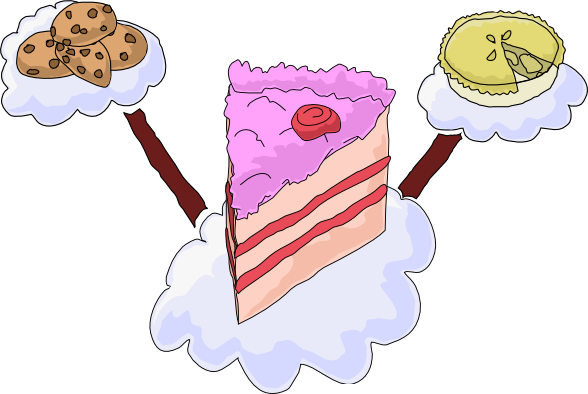
\includegraphics[scale=0.5]{images/sky_cake.png}

\end{center}
\end{frame}

\begin{frame}
\frametitle{zing server}

\huge
just hack up a server
\newline

\normalsize
\fbox{
    \lstinputlisting{code/zing/server.js}
}

\end{frame}

\begin{frame}
\frametitle{zing client}

\huge
then call the server's .zing() in your client!
\newline

\normalsize
\fbox{
    \lstinputlisting{code/zing/client.js}
}
\end{frame}

\begin{frame}
    \frametitle{none of this noise}
    
    \begin{columns}[c]
    \column{.2\textwidth}
        
\includegraphics[scale=0.4]{images/no.png}
    \column{.8\textwidth}
        \huge
        \begin{itemize}
            \item No schemas
            \item No XML
            \item No custom dispatching
        \end{itemize}
        \pause
        Just call functions!
    \end{columns}
\end{frame}

\begin{frame}
    \frametitle{client and server side by side}
    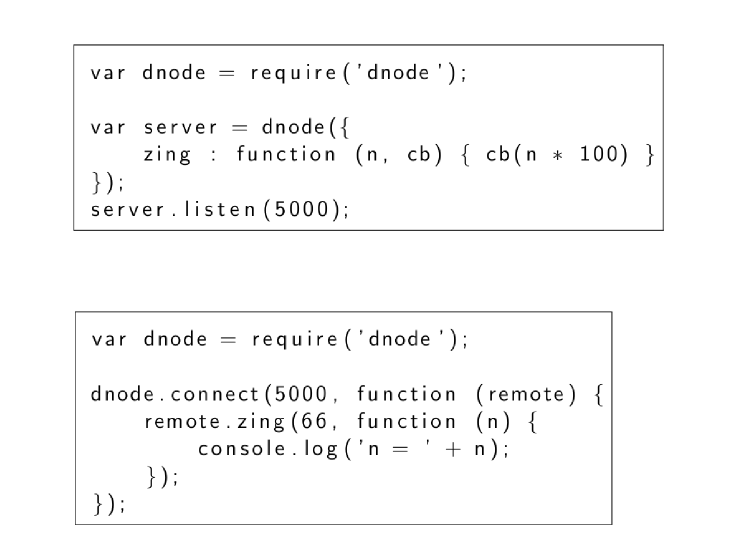
\includegraphics[scale=0.6]{images/zing_flow_0.png}
\end{frame}

\begin{frame}
    \frametitle{pass along n...}
    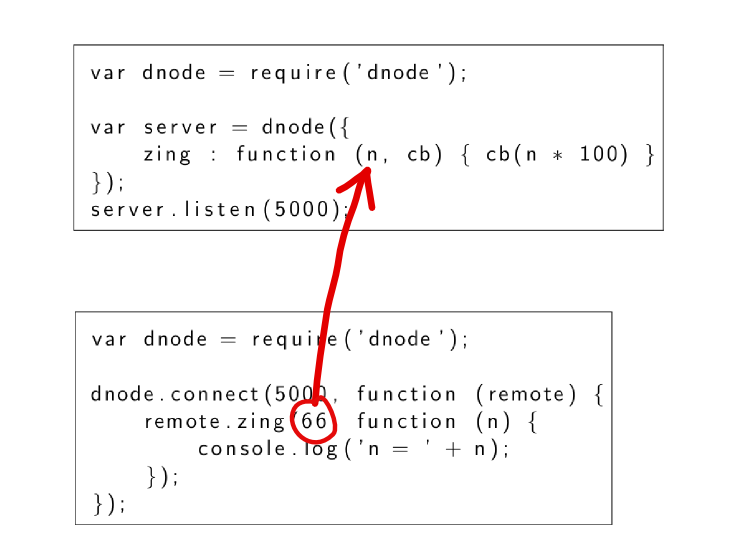
\includegraphics[scale=0.6]{images/zing_flow_1.png}
\end{frame}

\begin{frame}
    \frametitle{pass along the cb...}
    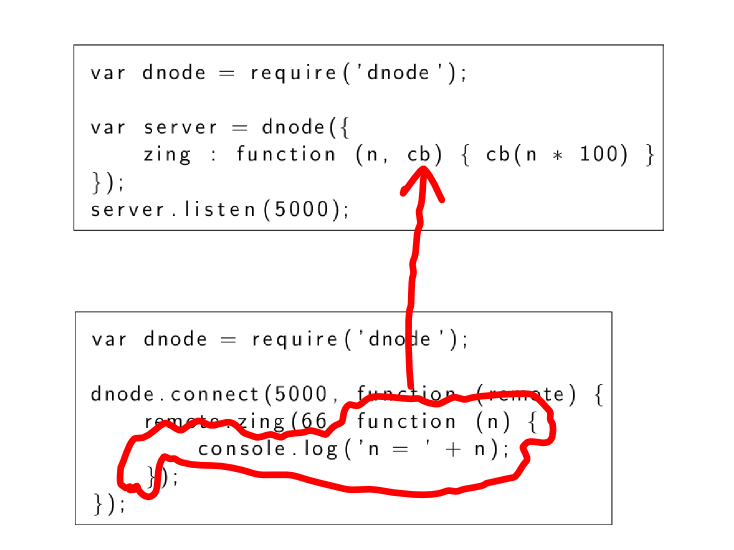
\includegraphics[scale=0.6]{images/zing_flow_2.png}
\end{frame}

\begin{frame}
    \frametitle{then just call the cb...}
    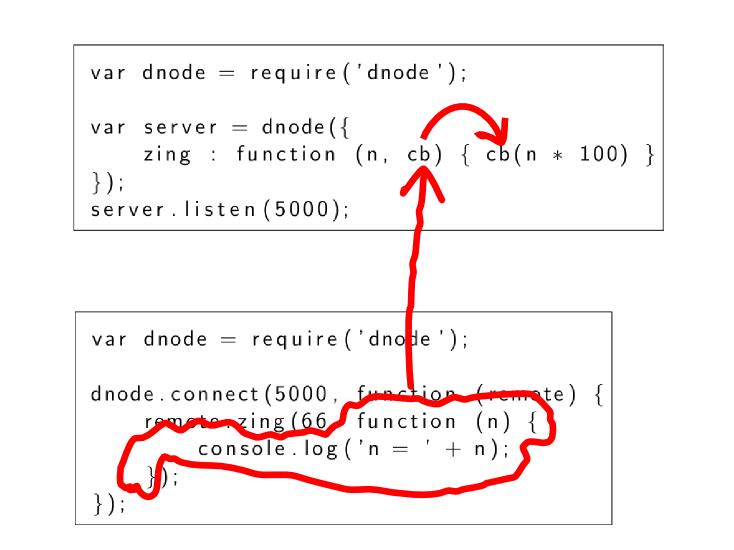
\includegraphics[scale=0.6]{images/zing_flow_3.png}
\end{frame}

\begin{frame}
    \frametitle{with the parameters you passed in...}
    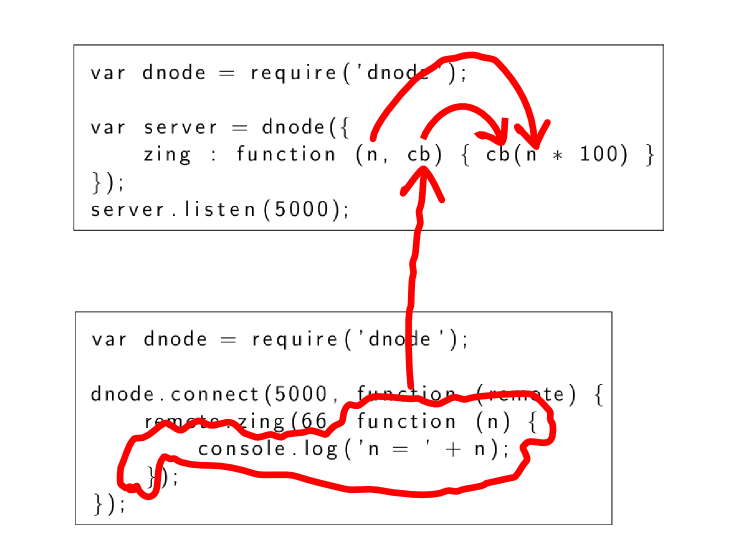
\includegraphics[scale=0.6]{images/zing_flow_4.png}
\end{frame}

\begin{frame}
    \frametitle{and your callback gets the result...}
    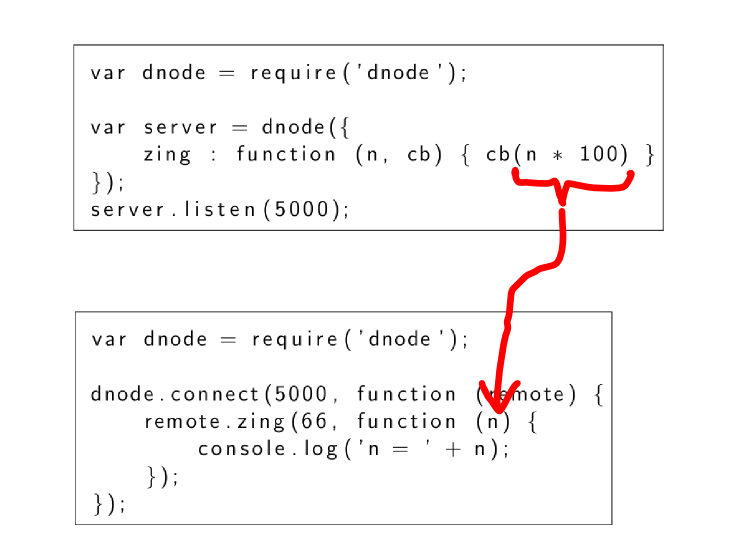
\includegraphics[scale=0.6]{images/zing_flow_5.png}
\end{frame}

\begin{frame}
    \frametitle{which you can use for whatevs}
    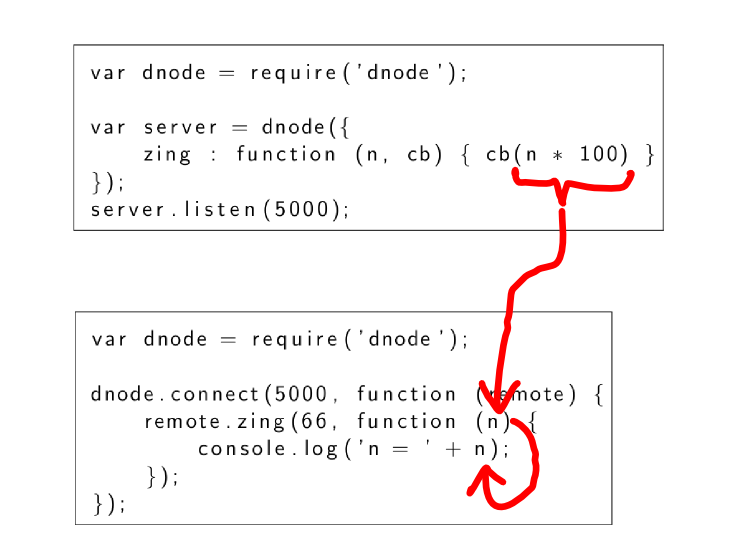
\includegraphics[scale=0.6]{images/zing_flow_6.png}
\end{frame}

\begin{frame}
    \frametitle{that's all it takes!}
    \begin{center}
        \fbox{\lstinputlisting{code/zing/output}}
    \end{center}
\end{frame}

\begin{frame}
    \frametitle{fuck yeah, callbacks!}
    \begin{center}
        
\includegraphics[scale=0.5]{images/fuck_yeah.png}
    \end{center}
\end{frame}

\begin{frame}
    \frametitle{callbacks fo' real}
\end{frame}

\end{frame}

\frame{
    and you can pass callbacks to your callbacks!
}

\frame{
    \begin{columns}[c]
    \column{.3\textwidth}
        
\includegraphics[scale=0.35]{images/all_the_way_down.png}
    \column{.7\textwidth}
        \begin{center}
        \huge
        It's callbacks all the way down.
        \end{center}
    \end{columns}
}

\frame{
    You can pull the same trick in the browser.
}

\frame{
    \frametitle{Git it!}
    {
        \begin{center}
        \huge
        github.com/substack/dnode
        \end{center}
    }
}

\end{document}
